% Created 2016-08-29 Mon 10:01
\documentclass[presentation]{beamer}
\usepackage[utf8]{inputenc}
\usepackage[T1]{fontenc}
\usepackage{fixltx2e}
\usepackage{graphicx}
\usepackage{grffile}
\usepackage{longtable}
\usepackage{wrapfig}
\usepackage{rotating}
\usepackage[normalem]{ulem}
\usepackage{amsmath}
\usepackage{textcomp}
\usepackage{amssymb}
\usepackage{capt-of}
\usepackage{hyperref}
\usepackage{minted}
\institute{Manipal Institute of Technology}
\usefonttheme[onlymath]{serif}
\usetheme{metropolis}
\setsansfont{Fira Sans}
\author{Pawan Dubey}
\date{\today}
\title{An Efficient URL-Pattern Based Algorithm for Accurate Web Page Classification}
\subtitle{CSE Seminar, 2016}
\hypersetup{
 pdfauthor={Pawan Dubey},
 pdftitle={An Efficient URL-Pattern Based Algorithm for Accurate Web Page Classification},
 pdfkeywords={},
 pdfsubject={},
 pdfcreator={Emacs 24.5.2 (Org mode 8.3.5)}, 
 pdflang={English}}
\begin{document}

\maketitle

\section{Preamble}
\label{sec:orgheadline4}
\begin{frame}[label={sec:orgheadline1}]{Authors}
Yiming Yang, Lei Zhang, Guiquan Liu, Enhong Chen at the University of Science and Technology of China
\end{frame}
\begin{frame}[label={sec:orgheadline2}]{Motivation}
\begin{itemize}
\item The paper proposes an efficient algorithm to classify web pages based on nothing but their URLs.
\item Presented at the 12th International Conference on Fuzzy Systems and Knowledge Discovery, 2015
\end{itemize}
\end{frame}
\begin{frame}[label={sec:orgheadline3}]{Colophon}
\begin{itemize}
\item Made with \(\LaTeX\) version 3.1415926. Presented with \alert{Beamer}
\item Source available at \url{http://github.com/pawandubey/seminar}
\end{itemize}
\end{frame}

\section{Introduction}
\label{sec:orgheadline8}

\begin{frame}[label={sec:orgheadline5}]{Web Page Classification}
\begin{itemize}
\item Assigning web pages to one of the predefined categories

\item Difficult because of the amount of data

\item Useful for contexual action
\end{itemize}
\end{frame}

\begin{frame}[label={sec:orgheadline6}]{State of the Art}
\begin{itemize}
\item Reading page text, hyperlinks etc

\item Natural Language Processing techniques on the page text
\end{itemize}

\begin{block}{\alert{Problems}}
\begin{itemize}
\item Too slow and inefficient

\item Complicated models
\end{itemize}
\end{block}
\end{frame}

\begin{frame}[label={sec:orgheadline7}]{URL Based Approach}
\begin{block}{URLs are the cheapest to access}
\begin{itemize}
\item Speed boost
\item Many relevant features due to SEO
\end{itemize}
\end{block}

\begin{block}{Current Methods}
\begin{itemize}
\item Use the same content-based techniques
\item No incremental learning methods
\end{itemize}
\end{block}
\end{frame}

\section{Background on URL Patterns}
\label{sec:orgheadline12}

\begin{frame}[fragile,label={sec:orgheadline9}]{URL-Patterns}
 \alert{What are URL Patterns?}
A regular expression matching the URLs of a group of related pages.
\begin{itemize}
\item \texttt{http://manipal.edu/*} matches all pages related to Manipal University
\item \texttt{http://manipal.edu/mit/*} matches all pages related to MIT, Manipal
\end{itemize}
\end{frame}

\begin{frame}[fragile,label={sec:orgheadline10}]{Pattern Tree}
 A \alert{\texttt{Suffix Tree}} like structure, instead for regexes.

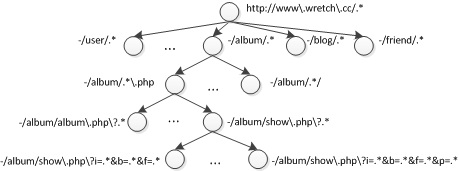
\includegraphics[width=.9\linewidth]{./website_structure_mining-pattern_tree.jpg}
\end{frame}

\begin{frame}[label={sec:orgheadline11}]{Pattern Tree Node}
Each node contains a key-value representation of the decomposed components of the URLs that matches the corresponding regex.

\alert{Example}
\emph{\url{https://google.com/search?q=regex}}
\begin{itemize}
\item \emph{Protocol} : HTTPS
\item \emph{Authority} : google.com
\item \emph{Path} : /search
\item \emph{q} : regex
\end{itemize}
\end{frame}

\section{The Algorithm}
\label{sec:orgheadline20}

\begin{frame}[label={sec:orgheadline13}]{Pattern Tree Construction}
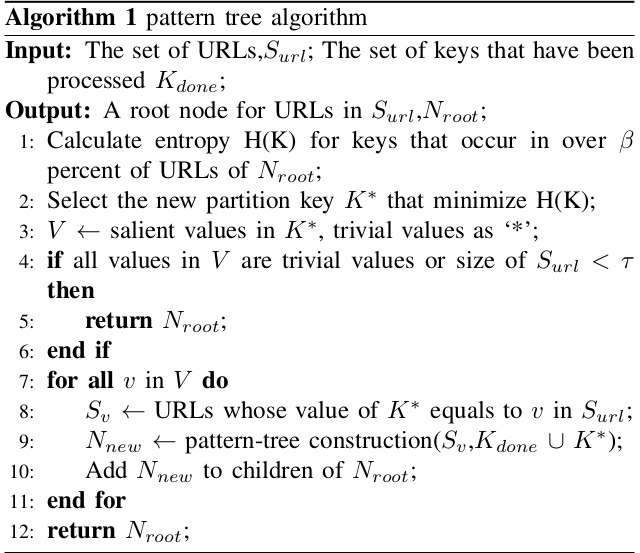
\includegraphics[width=.9\linewidth]{./pattern_algo1.png}
\end{frame}

\begin{frame}[label={sec:orgheadline14}]{Pattern Tree Construction}
\begin{itemize}
\item For each key decomposed from the URL set, we determine entropy
\end{itemize}

\alert{Shanon Entropy}
\begin{equation}
H(K) = \sum_{i=1}^{T} \frac{n_i}{N} log \frac{n_i}{N}
\end{equation}

We choose the \(K^*\) which minimizes this value as the splitting variable.
\end{frame}

\begin{frame}[label={sec:orgheadline15}]{Pattern Tree Construction}
\begin{itemize}
\item We select all values for the key \(K^*\) and divide them as \alert{salient} or \alert{trivial}
\item Division based on probablistic methods to find the \alert{decline} of the frequency
\item Recursively apply for all \alert{salient} values of \(K^*\)
\item Stop if either only \alert{trivial} values left or number of URLs less than threshold
\end{itemize}
\end{frame}

\begin{frame}[label={sec:orgheadline16}]{Problems}
\begin{itemize}
\item Recursive - inefficient
\item Not incremental
\end{itemize}

\alert{Improvement}
\begin{itemize}
\item An incremental modification to the algorithm
\end{itemize}
\end{frame}

\begin{frame}[label={sec:orgheadline17}]{Incremental Pattern Tree Construction}
\begin{itemize}
\item Only reconstruct tree if the \(K^*_{new}\) is different from \(K^*_{old}\)
\item Check if the new URLs match an existing node
\item If yes, add to matching node and recursively update
\item Create new nodes only if no match found for new URLs
\end{itemize}

\alert{Pros}
\begin{itemize}
\item Only update a subtree of the whole tree
\end{itemize}
\end{frame}

\begin{frame}[label={sec:orgheadline18}]{Pattern Generation}
\begin{itemize}
\item Relationship between keys are determined
\item Pattern is generated by topologically sorting the set of keys
\item Final pattern set is constructed by looking at the patterns of leaf nodes
\end{itemize}
\end{frame}

\begin{frame}[label={sec:orgheadline19}]{Classification}
\begin{block}{Binary}
\begin{itemize}
\item Pattern for only one of the classes are matched with the URL
\item Useful for tasks like sentiment analysis
\end{itemize}
\end{block}

\begin{block}{MultiClass}
\begin{itemize}
\item Patterns for all classes generated in advance
\item Pattern weight \(w_{ij}\) determines class of URL
\item \(w_{ij}\) is the number of URLs matching \(pattern_j\) in \(class_i\)
\item The longest matching pattern for the URL with each \(class_i\) is selected as \(candidate_i\)
\end{itemize}
\begin{equation}
label_{url} = \underset{i \in class_m}{max}(w_{candidate_i})
\end{equation}
\end{block}
\end{frame}

\section{Evaluation}
\label{sec:orgheadline25}
\begin{frame}[label={sec:orgheadline21}]{Performance Measures}
In terms of Information Retrieval, if the problem is to retrieve relevant documents from a dataset,
\begin{itemize}
\item \alert{Precision} is the fraction of retrieved documents which are relevant
\item \alert{Recall} is the fraction of relevant documents that are retrieved
\item \alert{F1 score} is the harmonic mean of \alert{precision} and \alert{recall}
\end{itemize}
\begin{equation}
F1 = 2 \cdot{} \frac{precision \cdot recall}{precision + recall}
\end{equation}
\begin{itemize}
\item Running Time
\end{itemize}
\end{frame}

\begin{frame}[label={sec:orgheadline22}]{Setup}
\begin{itemize}
\item WebKB dataset
\item Comparison with \emph{Web Classification Using N-gram Based URL Features} by \emph{R.Rajalakshmi}
\item And \emph{Rule Based Method}
\item 90-10 Training-Test split
\end{itemize}
\end{frame}

\begin{frame}[label={sec:orgheadline23}]{Functional Classification}
To validate effectiveness and efficiency in classification
\begin{block}{Results}
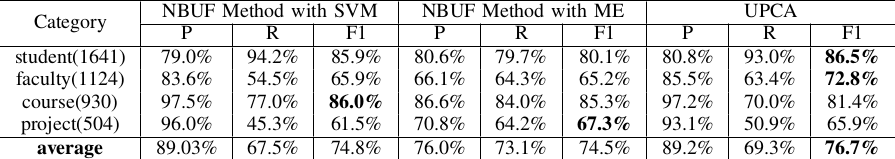
\includegraphics[width=.9\linewidth]{./fcl.png}
\end{block}
\begin{block}{Take aways}
\begin{itemize}
\item UPCA is about 10X faster than NBUF
\item Achieves an improvement of 2\% on F1
\item Performs better on larger datasets
\end{itemize}
\end{block}
\end{frame}

\begin{frame}[label={sec:orgheadline24}]{High Quality Page Identification}
Prove effectiveness on a dataset with much noise.
\begin{block}{Results}
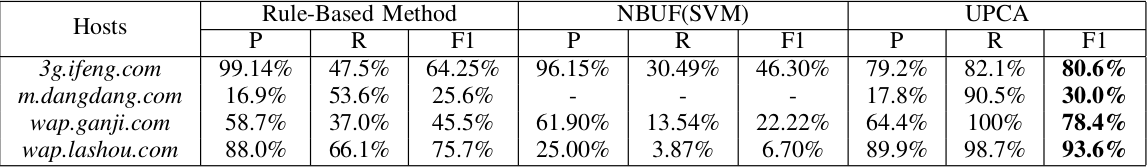
\includegraphics[width=.9\linewidth]{./rbm.png}
\end{block}
\begin{block}{Take aways}
\begin{itemize}
\item UPCA is clearly superior to the \emph{Rule Based Method} approach
\end{itemize}
\end{block}
\end{frame}

\section{Conclusion}
\label{sec:orgheadline27}
\begin{frame}[label={sec:orgheadline26}]{Performance Comparison}
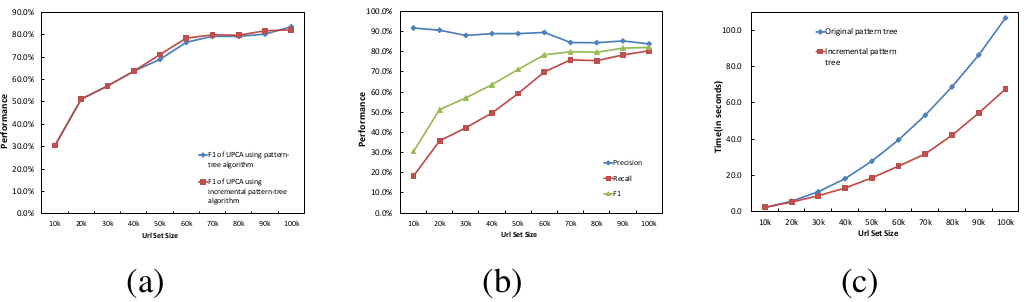
\includegraphics[width=.9\linewidth]{./upca.png}

\begin{itemize}
\item UPCA provides a much more efficient way to classify web pages based on URLs
\item The incremental algorithm achieves a performance gain on the recursive one
\item A distributed version required for processing very large data sets
\end{itemize}
\end{frame}

\section{Resources and References}
\label{sec:orgheadline29}
\begin{frame}[label={sec:orgheadline28}]{References}
\begin{itemize}
\item Tao Lei, Rui Cai, Jiang-Ming Yang, Yan Ke, Xiaodong Fan, Lei Zhang. \emph{A Pattern Tree-based Approach to Learning URL Normalization Rules.} In Proc. of the 19th International World Wide Web Conference (WWW 2010)

\item Y. Lin, T. Zhu, X. Wang, J. Zhang, and A. Zhou. \emph{Towards online review spam detection.} In WWW, pages 341–342. IW3C2, 2014.

\item R. Rajalakshmi and C. Aravindan. \emph{Web page classification using n-gram based url features.} In Advanced Computing (ICoAC), pages 15–21. IEEE, 2013.
\end{itemize}
\end{frame}
\end{document}
